% Inicio del preámbiulo

\documentclass[letterpaper,12pt]{article} %Modifica el tipo de documento y el tamaño de la letra.
\usepackage[utf8]{inputenc} %Formato UTF-8 para caracteres especiales.
\usepackage[shortlabels]{enumitem}
\usepackage[spanish,mexico]{babel} 
\usepackage{amsmath,amssymb,amsfonts,latexsym,cancel}
\usepackage{hyperref}
\usepackage{wrapfig}
\usepackage[rflt]{floatflt}
\usepackage[pdftex]{graphicx}
\usepackage{fancyhdr} %Paquete para el header y el formato de la portada. No sugiero borrarlo!
\usepackage{float}
\usepackage{longtable,multirow,booktabs}
\usepackage{cite}
\usepackage{wrapfig}
\usepackage[square,numbers]{natbib}
\usepackage{multicol}
\usepackage{caption}
\usepackage[]{sidecap}
\usepackage{adjustbox}
\usepackage{parskip}
\usepackage{enumitem}
\usepackage{tikz}
\usepackage{lipsum}
\usepackage[]{xcolor}

%Fin de Préambulo

% Variables del documento
% Document Variables 
\newcommand{\myMateria}{Técnicas y Herramientas modernas}
\newcommand{\myGrupo}{ "Linces"}
\newcommand{\mySemester}{2024}
\newcommand{\MyReport}{Vinventions}
\newcommand{\myUnidad}{"Módulo especial Sitevinitech"}
\newcommand{\myDate}{5 de junio de 2024}
\newcommand{\myName}{Emilia Gulle 13678, Martin Federico Herrera 13475, Delfina Di Paola 13740, Lucía Boscafiori 13734, 
Guadalupe Gual 13807 y Maria Paz Antich 13728}
\newcommand{\myTeacher}{PALMA, Ricardo Raúl }



%Inicio formato de Página. 

\textheight = 21cm %Medidas de la  página
\textwidth = 18cm  %Medidas de la página
\topmargin = -2cm  %Medidas de la página    
\oddsidemargin = -0.8cm %Medidas de la página
\pagestyle{fancy} %Diseño de la página

\fancyhf{}
\lhead{\myMateria}%%LeftHead
\rhead{
\includegraphics[ height=1cm]{Imágenes/uncufing.png}}%%CenterHead
%\lfoot{USM}


\setlength{\columnsep}{4mm}%Comandos para el formato de la página.
%\setlength{\parindent}{4em}%Sangría al comenzar un nuevo párrafo.
\setlength{\parindent}{0.5in}
%\setlength{\parindent}{4em}%Sangría al comenzar un nuevo párrafo.
\setlength{\parskip}{1em}%Distancia entre párrafos.
\renewcommand{\baselinestretch}{1.0}% Espacio entre línea y línea o interlineado.
\setlength{\headheight}{33pt}
\fancyfoot[C,CO]{\thepage} %Logo de LaTeX y pie de página.

%Fin formato de Página

%Aquí inicia el documento.

\begin{document}

    %LaTeX te hace el índice automáticamente conforme añades secciones en tu documento.
    \thispagestyle{empty}
			\begin{figure}[ht]
		   \minipage{0.7\textwidth}
				
\includegraphics[width=5cm]{Imágenes/logouncuyo.png}
				\label{escudoTecNM}
		   \endminipage
		   \minipage{\textwidth}
				
\includegraphics[width=5cm]{Imágenes/fing.png}
				\label{EscudoITCJ}
			\endminipage
				%%\vspace{-1cm}
		\end{figure}
		
		\vspace{0.1cm}
		
		\begin{center}
		    {\scshape\LARGE \textbf{ UNIVERSIDAD NACIONAL DE CUYO} \par}
			{\scshape\Large Facultad de Ingeniería \par}
			{\scshape\large Ingeniería Industrial \par}
            \vspace{0.75cm}
             {\Large \textbf{\myMateria}}

			% Restauramos el interlineado:
			\begin{center}
			
			
			{\Large Grupo:\myGrupo}
			\vspace{0.75cm}
				
			{\LARGE\bfseries \MyReport\\Unidad \myUnidad\par}
            \vspace{0.75cm}
            
		{\scshape\Large Fecha de entrega: \myDate\par}	
        \vspace{0.75cm}
	    \LARGE	{ \textbf{Profesor: }}\\
        \large		{ \myTeacher}
        
		\vspace{0.5cm}	
		
		\LARGE	{ \textbf{Alumno:}}
        
        \normalsize	 {\myName}

%% \it es letra itálica
				\vspace{1.25cm}
				\vspace{0.9cm}
				
			\end{center}
	
		\end{center}
    \newpage
    \tableofcontents
    \newpage
%Inicio parte opcional. Esta parte la puedes quitar si deseas, es por si te piden formatos para
%evidencias de certificación de los laboratorios con números de cuenta o te piden abstracts en tus %trabajos.

\title{\myMateria \\\textbf{\MyReport} \\ } 

\author{ \normalsize{\texttt{\myGrupo}} }
\date{\myDate}
\maketitle
\thispagestyle{fancy}

\begin{abstract}
El día viernes 17 de Mayo pudimos asistir a la feria "Sitevinitech", en donde tuvimos la oportunidad de hablar con importantes expositores de la misma, entre ellos el CEO de "Vinventions Latinoamérica". 
\end{abstract}

%Fin parte opcional

\section{Introducción}

\noindent Como se mencionó previamente, pudimos asistir a la feria "Sitevinitech 2024". Realizamos el recorrido completo de la misma, pasando por los stands de más de 100 expositores. Le realizamos una entrevista a Andrés Belinsky, CEO de Vinventions Latinoamerica. A continuación, se encuentra más información sobre la feria y sobre Vinventions. 

\section{Sitevinitech: Origen e Historia}
Sitevinitech es una feria internacional dedicada a la vitivinicultura y las tecnologías asociadas a la industria del vino, frutas y verduras. Es una plataforma donde se reúnen profesionales del sector para intercambiar conocimientos, presentar innovaciones y establecer redes de contactos.

Sitevinitech se originó a partir de Sitevi, una feria dedicada principalmente a la vitivinicultura. A medida que creció, se expandió para incluir tecnologías para la producción de frutas y verduras, convirtiéndose en una referencia global para la agroindustria.

Aunque la edición principal se celebra en Montpellier, Francia, Sitevinitech también se ha extendido a otros países, especialmente en América Latina y Asia, reflejando su alcance global y la importancia de estos mercados emergentes.

Sitevinitech ha consolidado su presencia global, convirtiéndose en un evento crucial para la vitivinicultura y la agroindustria en diversas regiones del mundo. Su capacidad para reunir a expertos, presentar innovaciones y facilitar redes de contacto hace que sea una feria indispensable para los profesionales del sector.


\section{Sitevinitech Argentina 2024}

"Sitevinitech Argentina" es la feria más importante de la Industria Vitivinícola y Agrícola de Latinoamérica. La primera edición en Argentina tuvo lugar en 2014 y se lleva a cabo en la provincia de Mendoza.

Esta feria internacional contó con un enorme número de stands de distintas empresas, emprendimientos, así como también exposiciones sobre proyectos sustentables y tecnología para el agro. Durante los tres días se desarrollaron rondas de negocios internacionales, ciclos de charlas y conferencias, demostraciones de firmas regionales,  premiaciones y concursos de degustación. 

 Esta feria se ha convertido en la exhibición referente para Latinoamérica en el mundo vitivinícola, abriendo oportunidades en el mercado europeo para las empresas locales. \\
 
La misma contó con:
\begin{itemize}
\item 10.000m2
\item 150 expositores
\item 10.000 visitantes
\item Más de 10 países participantes
\end{itemize}

\begin{figure}[h]
    \centering
    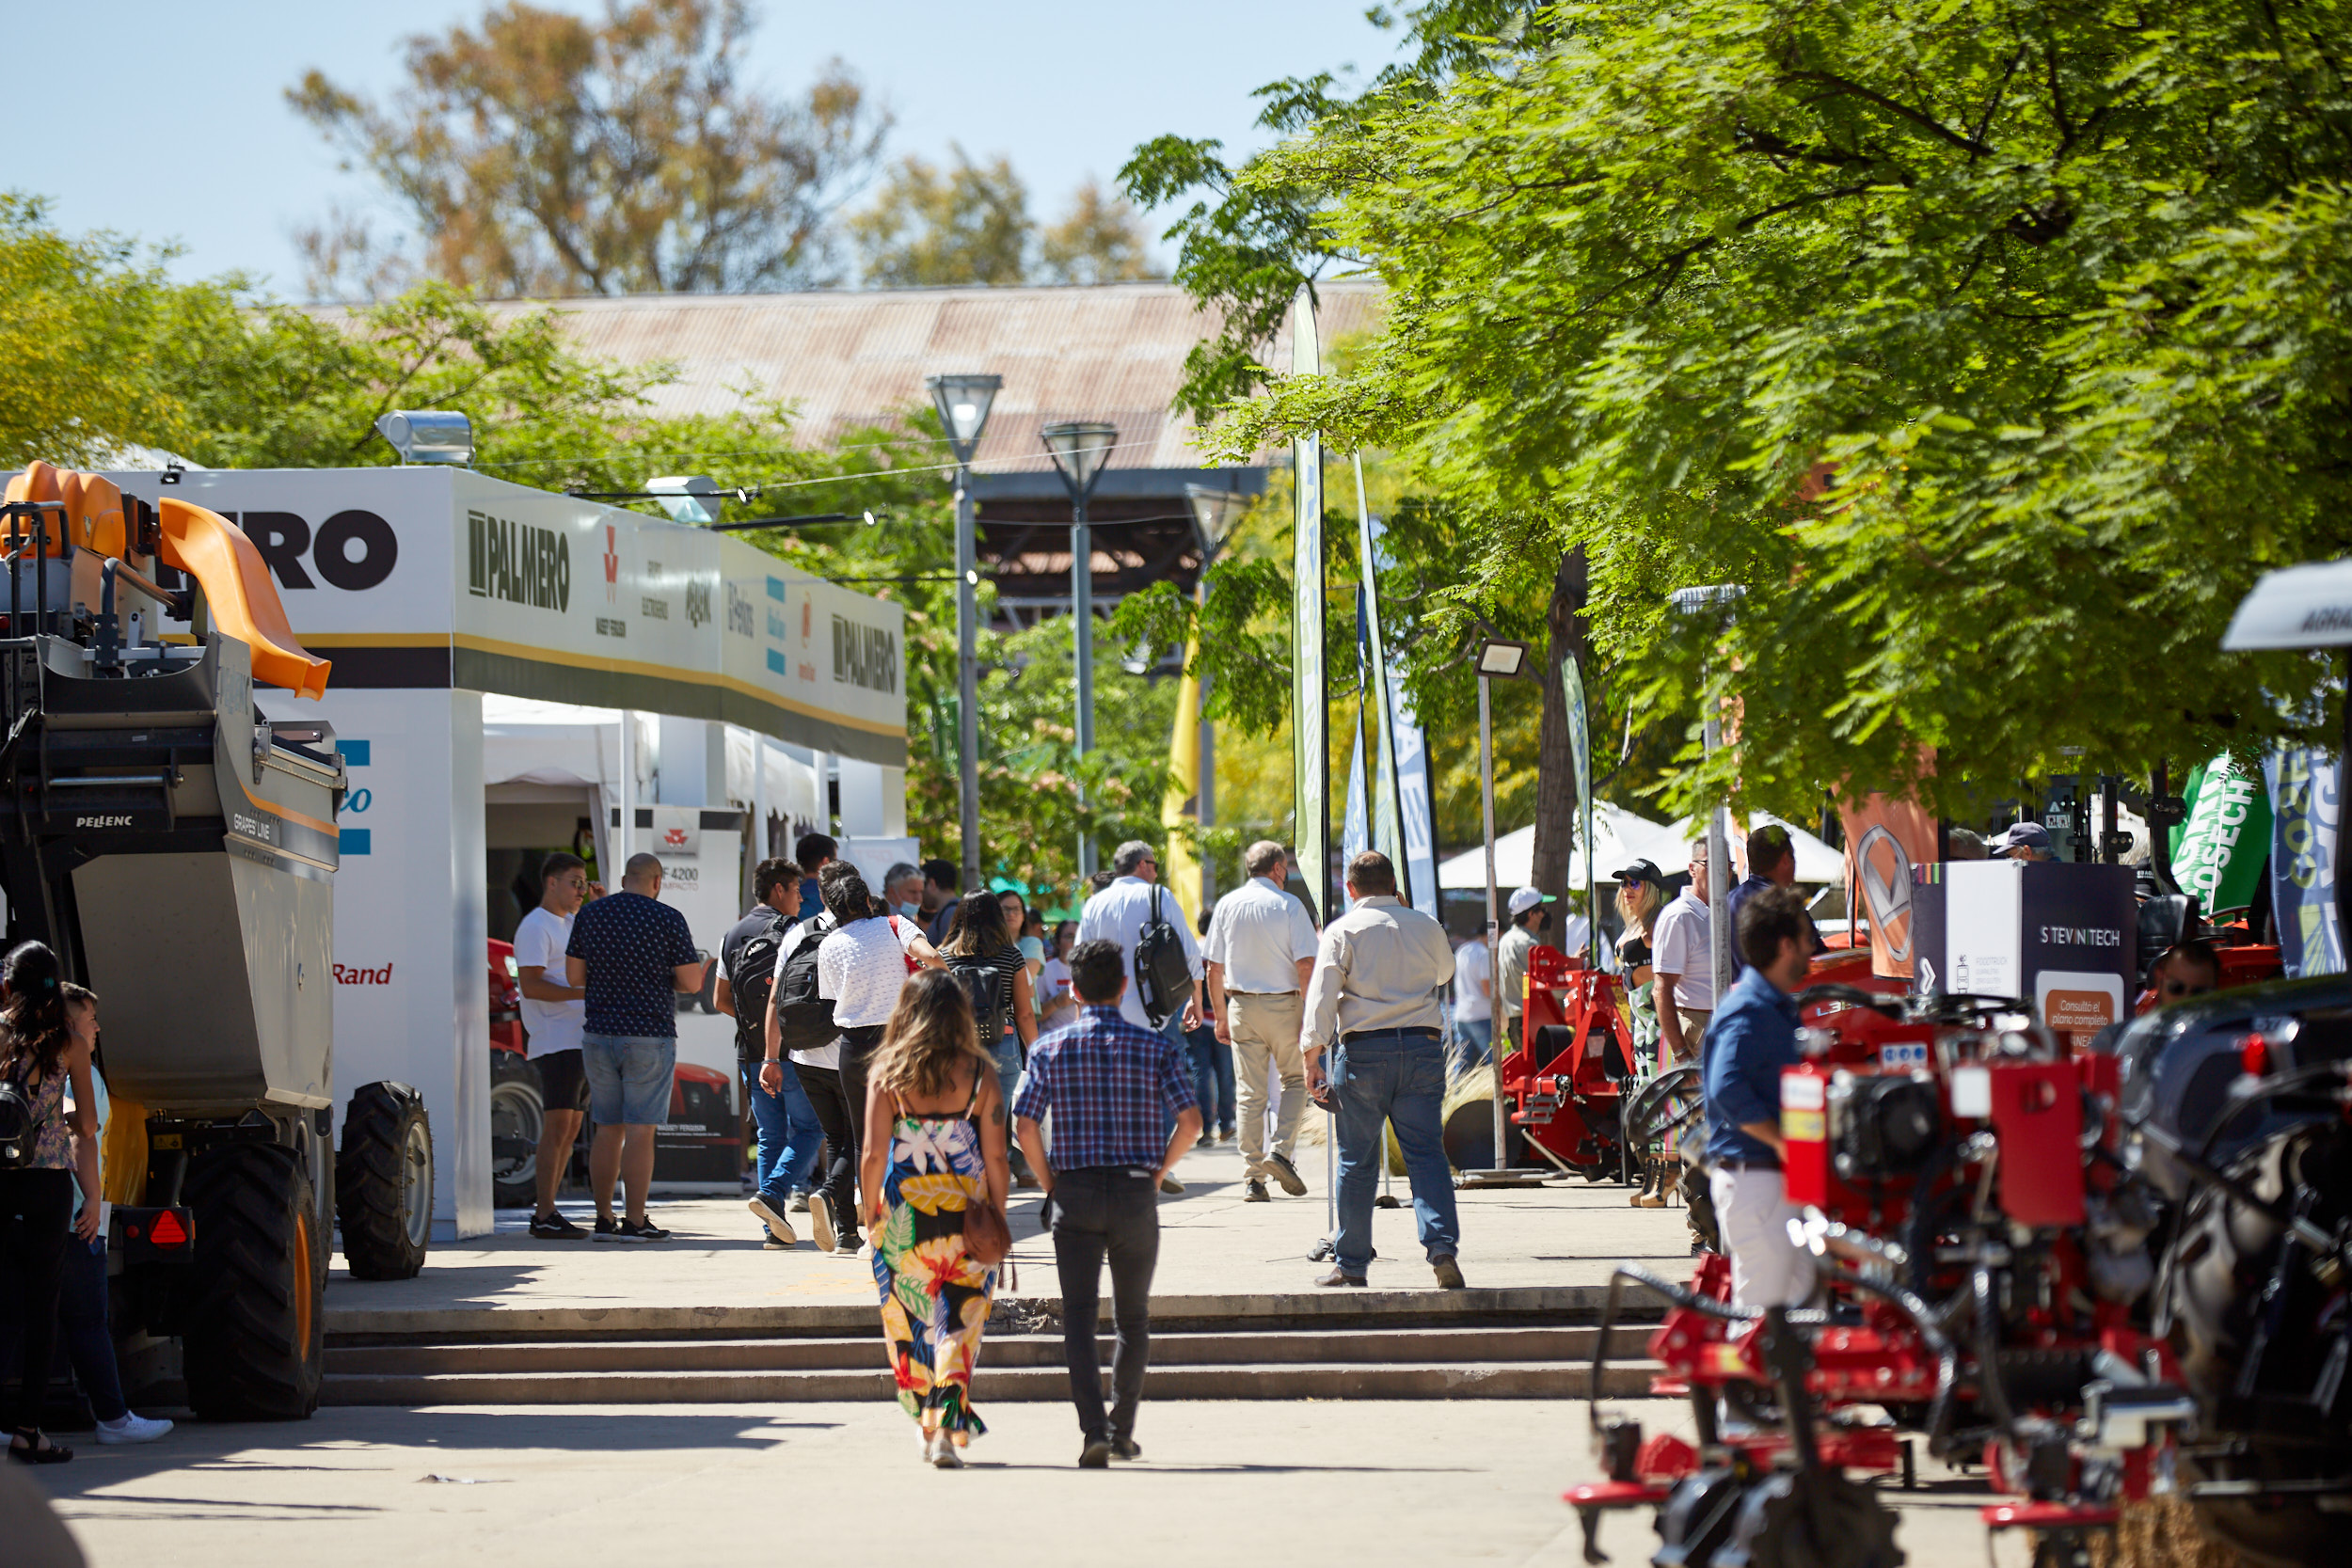
\includegraphics[height=7cm]{Imágenes/Sitevinitech.png}
\end{figure}

\section{Vinventions}

Vinventions es una empresa global que se especializa en soluciones de cierre para la industria del vino. Fundada en 2015, Vinventions ofrece una gama de productos y servicios diseñados para preservar la calidad del vino y mejorar la experiencia del consumidor.

Una de las innovaciones clave de Vinventions es la capacidad de sus cierres para controlar la cantidad de oxígeno que entra en la botella, lo que ayuda a mantener la calidad del vino durante su almacenamiento y envejecimiento.

Se compromete con la sostenibilidad, utilizando materiales reciclables y de origen vegetal en sus productos, y promoviendo prácticas de producción ecológicas.
\begin{figure}[h]
    \centering
    
\includegraphics[height=4cm]{Imágenes/vin3.png}
\end{figure}


\section{Entrevista a Andrés Belinsky}

Durante la feria, Sitevinitech, pasamos por el stand de Vinventions y tuvimos la oportunidad de conversar con Andres Belinsky, CEO de Vinventions Latinoamerica. 

El mismo, explicó que la participación de la empresa en la feria Sitevinitech responde a su interés de mostrar y comunicar las novedades a sus clientes, tanto locales como de otros países como Chile, Perú y Bolivia. Vinventions ha participado en varias ediciones de la feria y continúa haciéndolo debido al éxito en la generación de contactos y relaciones comerciales. A su vez, Vinventions es sponsor de la misma debido a que, como mencionó Andrés: " queremos lograr mayor visibilidad de nuestra empresa en el ámbito del mundo vitivinícola a nivel regional.  Y es una forma de apoyar a la feria que consideramos muy importante."


Por otro lado, la empresa líder en sistemas de cierre para vinos, compite con los demás sistemas de cierres, tanto de tapones sintéticos, como Tapi, o empresas locales que representan a corcheras de Portugal, como Amorim, Crok Supply o Portocork y también las de tapa a rosca, como Guala, Ramondin o Amcor.

Sin embargo, la misma, como nos comentó  su CEO, en los ultimos años ha logrado grandes innovacciones:

"Hemos logrado records de velocidad de producción en nuestra extrusora, innovando con el agregado de una quinta rueda para el proceso de enfriamiento, lo que nos permite aumentar la velocidad. También, hace unos años "creamos" una máquina junto a ingenieros de una empresa local en San Juan, que remplazaba dos máquinas que se usaban en otras filiales. Así, redujimos dos etapas en una sola, minimizando los tiempos del proceso, menos operarios y menor inversión de la máquina. Esta innovación se exportó luego a las fabricas de Bélgica, USA y China."
\begin{figure}[h]
    \centering
    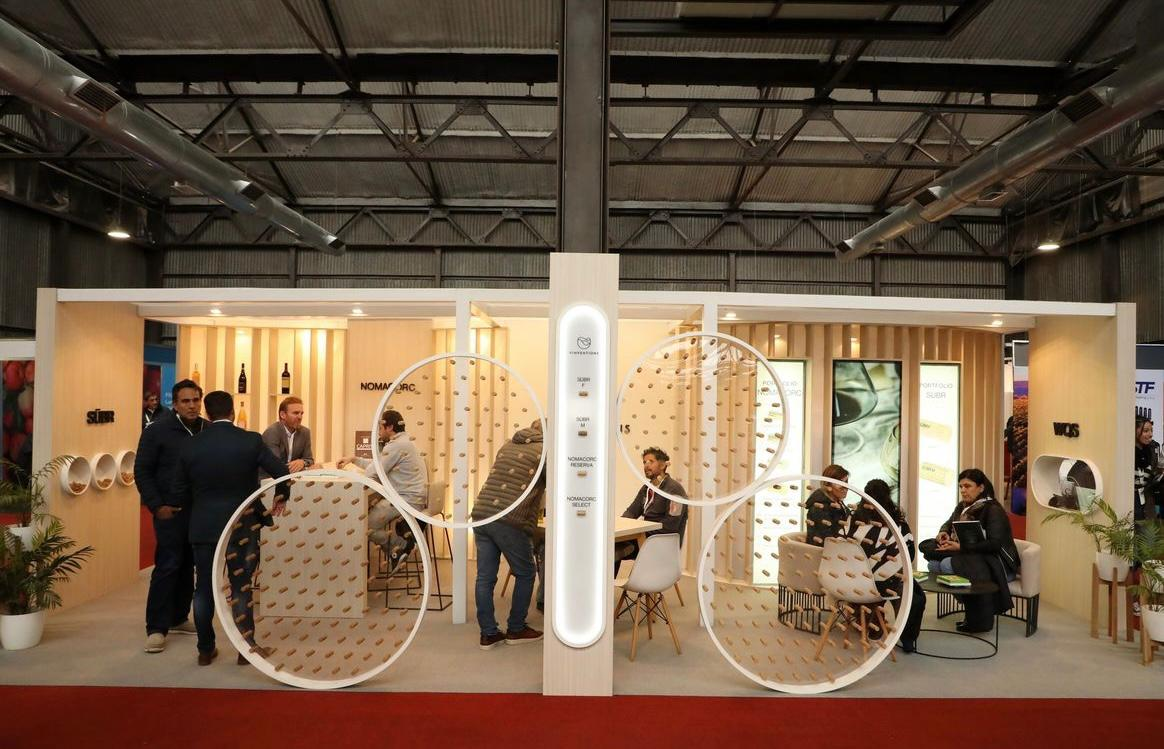
\includegraphics[height=7cm]{Imágenes/vinventions2.png}
\end{figure}

En cuanto a la sostenibilidad y la eficiencia de sus productos, Vinventions, desde sus inicios, con la marca Nomacorc en 1999, comenzó ofreciendo un producto reciclable. Con el tiempo, se han incorporado otras características y beneficios, como el uso de biopolietileno derivado de la caña de azúcar en su línea Nomacorc Green, lo que ha llevado a una muy baja o nula huella de carbono. Además, hace unos años lanzaron, en Europa, la versión Nomacorc Blue Line, que utiliza polietileno reciclado con un proceso que permite reciclarlo infinitamente y es técnicamente superior al reciclado mecánico.

Además, la empresa lanzó un corcho microaglomerado de la marca SÜBR, que utiliza como aglomerante un polímero biodegradable y evita el uso del pegamento de poliuretano utilizado por sus competidores. En la planta de San Juan, se ha logrado utilizar más del 70\% de energía eólica este año, con la meta de alcanzar el 100\% en un futuro cercano.

La empresa también hace un uso muy bajo de agua, y reutiliza la misma usándola varias veces en el proceso mediante un circuito cerrado. Posteriormente, este agua puede ser vertida en los cauces normales, dado que no está contaminada. En cuanto al proceso, se han logrado altos niveles de eficiencia, lo que permite minimizar el consumo de energía. Además, todo el scrap generado en el proceso se recicla.

\begin{figure}[h]
    \centering
    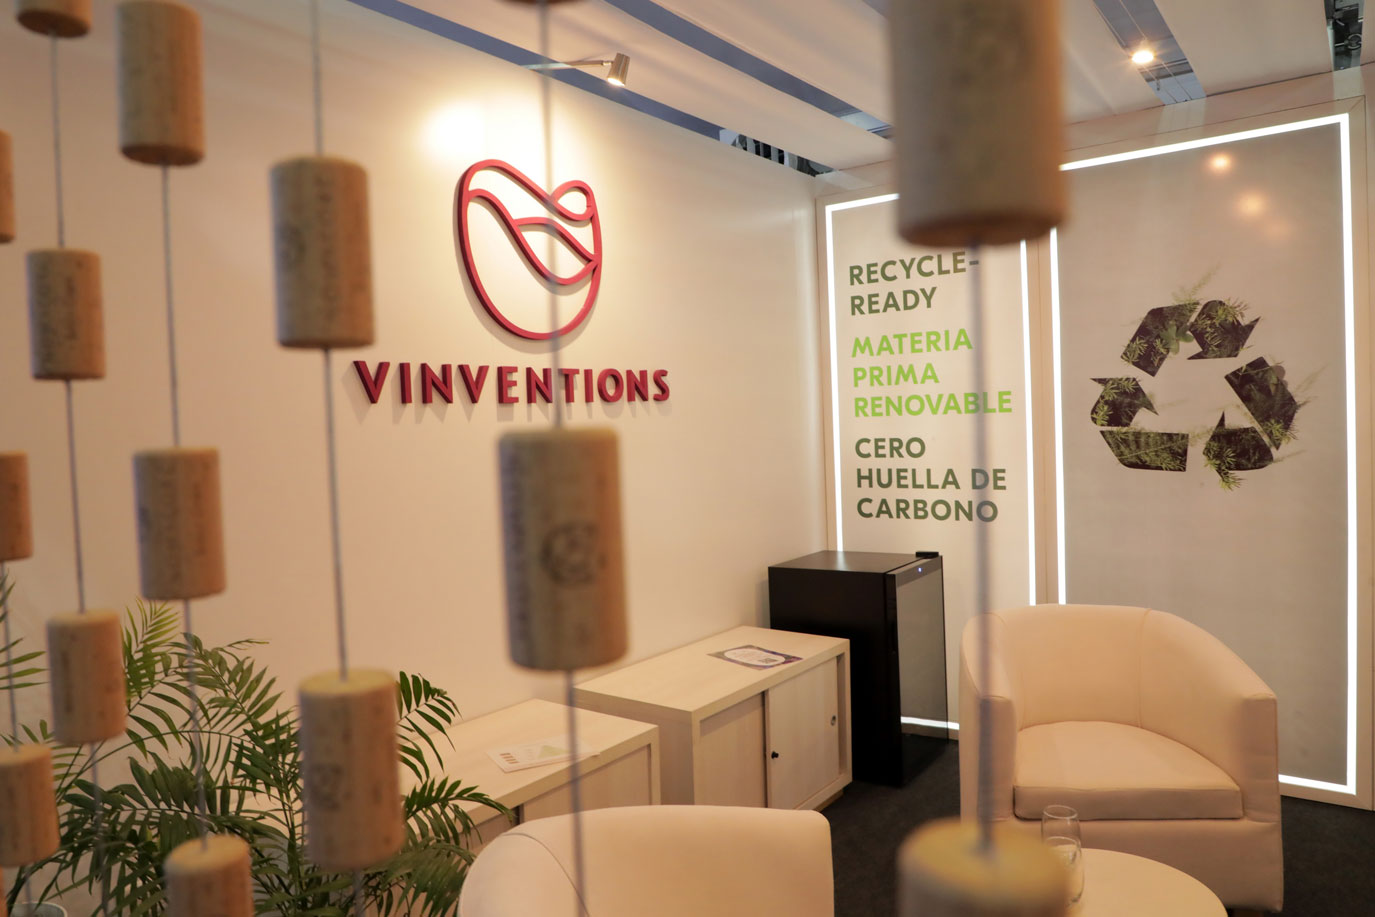
\includegraphics[height=7cm]{Imágenes/vinventions.png}
\end{figure}

Por utilmo, Andrés afirma que lo que los destaca en el mercado y su ventaja frente a sus competidores es: ``Confiabilidad para proteger al vino una vez embotellado, innovación permanente, características de sustentabilidad y precio competitivo.´´

 \section{Conclusión}
 
 La participación en la feria "Sitevinitech" el 17 de mayo proporcionó una valiosa oportunidad para interactuar con destacados expositores, incluyendo al CEO de una reconocida empresa Vinventions.

"Sitevinitech" se ha consolidado como una plataforma internacional crucial para la vitivinicultura y las tecnologías agrícolas. Originada a partir de "Sitevi", la feria ha ampliado su alcance a nivel global, siendo un referente no solo en Montpellier, Francia, sino también en América Latina y Asia.

La edición local, "Sitevinitech Argentina 2024", celebrada en Mendoza, reunió a un amplio número de expositores y empresas, ofreciendo una plataforma para la exhibición de productos, proyectos sustentables y tecnología agrícola.

Dentro de este contexto, la empresa líder en sistemas de cierre para vinos se destacó por su compromiso con la innovación y la sostenibilidad, implementando soluciones reciclables y avances significativos en materiales biodegradables y energías renovables.

En la entrevista con el CEO de la empresa, se resaltó su participación activa en la feria como una estrategia para comunicar sus novedades y fortalecer relaciones comerciales a nivel local e internacional, destacando su posición competitiva basada en la confiabilidad de sus productos, la innovación continua y su enfoque en la sustentabilidad.

 La experiencia en "Sitevinitech" permitió una inmersión completa en las tendencias, innovaciones y oportunidades que impulsan el desarrollo de la industria vitivinícola y agrícola, resaltando el papel crucial de eventos como este en la promoción del sector y la generación de sinergias entre actores clave.






\centering\vspace*{\fill} 
\end{document}

 %Fin del documento.